\documentclass[12pt, a4paper]{article}

% --- Core Packages ---
\usepackage[utf8]{inputenc}
\usepackage{geometry}
\geometry{a4paper, margin=2.5cm}
\usepackage{graphicx}
\usepackage{float}
\usepackage{hyperref}

\graphicspath{{../results/project/plots/}} % Adjusted to your folder structure

% --- Document Information ---
\title{Machine Learning and Pattern Recognition\\ \large Laboratory 04: Probability and Density Estimation}
\author{Nicola Beccaceci}
\date{}

\begin{document}

\maketitle

\section*{1D Gaussian Density Estimation}

In this laboratory, we fit uni-variate Gaussian models to the different features of the Fake (label 0) and Genuine (label 1) classes using Maximum Likelihood Estimation (MLE). By plotting the continuous Gaussian density curves on top of the normalized discrete histograms, we evaluate the validity of the Gaussian assumption for our dataset.

\subsection*{Question: What do you observe?}

\subsubsection*{Empirical results}
We observe a sharp dichotomy in the dataset's distributions. The majority of the features (Features 1 through 4) present a standard, unimodal geometry for both classes. However, Features 5 and 6 exhibit complex topological structures, breaking the standard normality assumption—most notably in the Genuine class, which displays distinct bimodal distributions.

\subsubsection*{Theoretical analysis}
The Maximum Likelihood Estimator attempts to find a single mean ($\mu$) and variance ($\sigma^2$) that maximizes the probability of observing the training data. For unimodal distributions, this optimization successfully centers the density over the data's center of mass. However, for multi-modal geometries, the MLE compromises by placing the mean directly between the modes, resulting in a severe mismatch between the theoretical model and the empirical reality.

\subsection*{Question: Are there features for which the Gaussian densities provide a good fit?}

\subsubsection*{Empirical results}
Yes, the 1D Gaussian model provides a highly accurate fit for **Features 1, 2, 3, and 4** across both the Fake and Genuine classes.

\begin{itemize}
    \item \textbf{Fake Class:} The empirical histograms for Features 1 through 4 are highly symmetric and unimodal. For example, Feature 1 (mean $0.0029$, variance $0.5696$) and Feature 4 (mean $0.6708$, variance $0.5360$) are perfectly wrapped by their estimated Gaussian curves.
    \item \textbf{Genuine Class:} Features 1 through 4 similarly exhibit strong symmetric distributions. Feature 3 (mean $0.6652$, variance $0.5489$) shows an excellent fit, with the empirical data smoothly following the theoretical exponential decay dictated by the Gaussian formula.
\end{itemize}

\subsubsection*{Theoretical analysis}
For these specific features, the underlying data generation process closely mimics a normal distribution. The lack of heavy skewness or multiple peaks means that the two parameters of the Gaussian model ($\mu$ and $\Sigma$) contain sufficient mathematical capacity to fully describe the class-conditional densities. 

\begin{figure}[H]
    \centering
    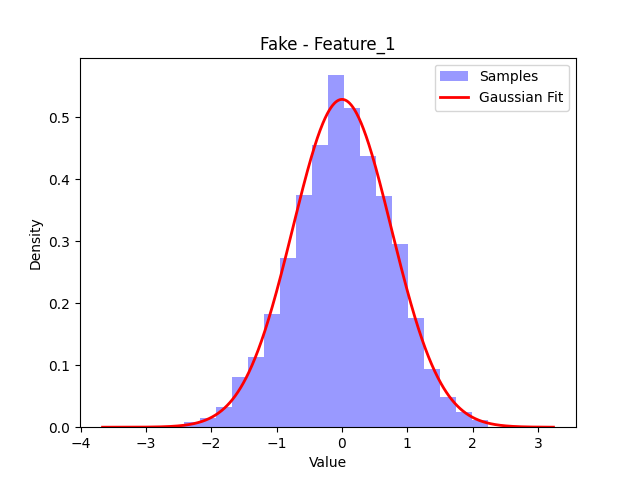
\includegraphics[width=0.48\linewidth]{fake_feature_1.png}
    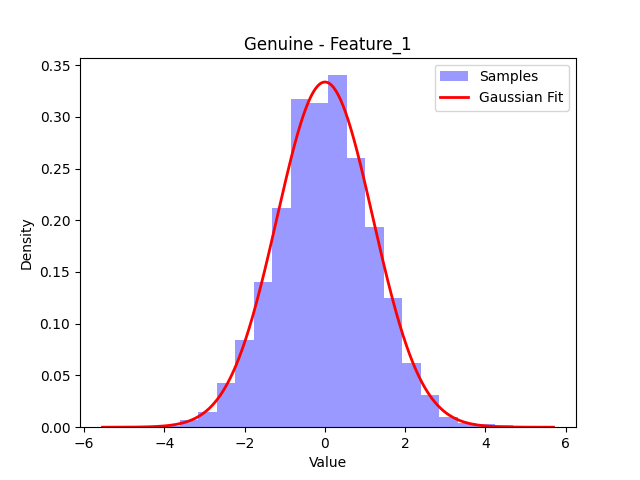
\includegraphics[width=0.48\linewidth]{genuine_feature_1.png}

    \vspace{0.3cm}
    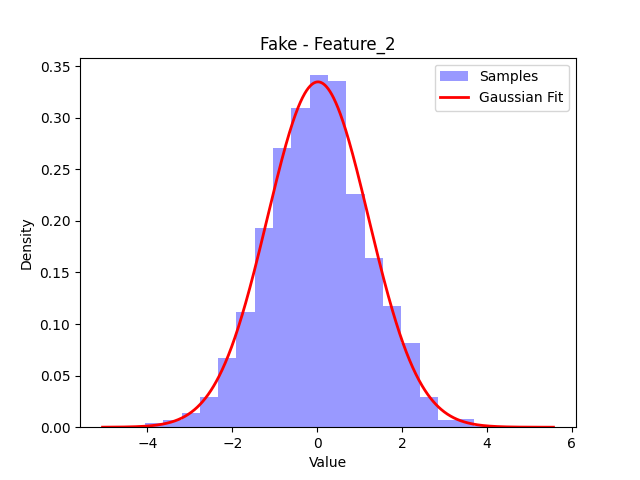
\includegraphics[width=0.48\linewidth]{fake_feature_2.png}
    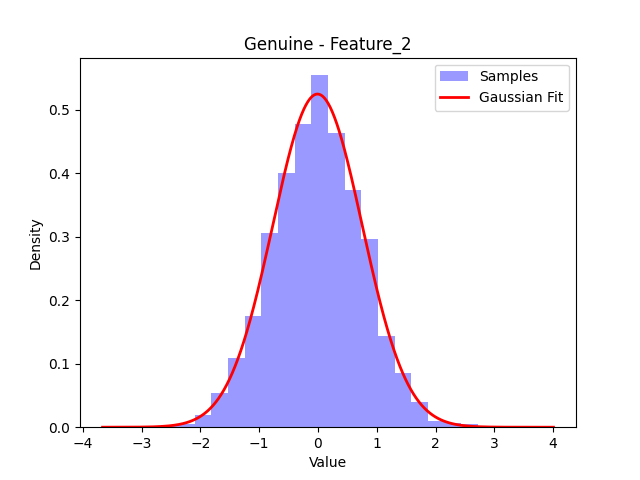
\includegraphics[width=0.48\linewidth]{genuine_feature_2.png}
    
    \vspace{0.3cm}
    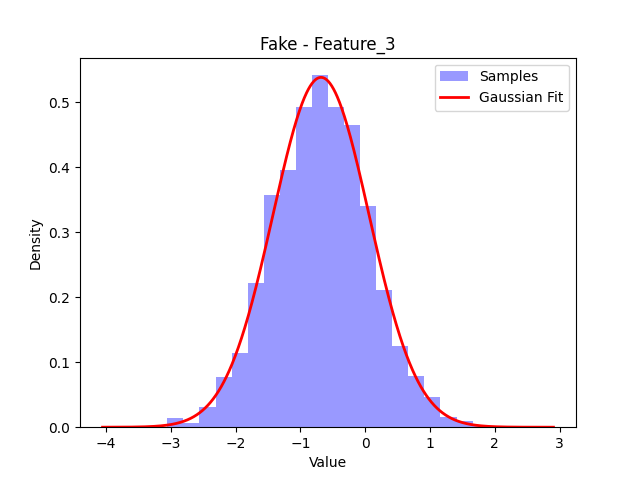
\includegraphics[width=0.48\linewidth]{fake_feature_3.png}
    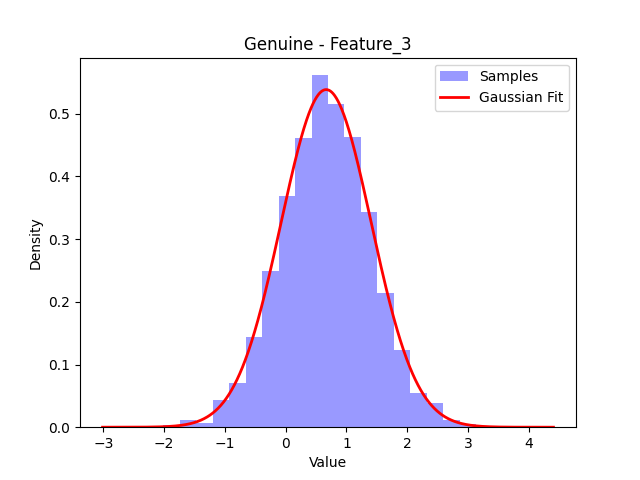
\includegraphics[width=0.48\linewidth]{genuine_feature_3.png}

    \vspace{0.3cm}
    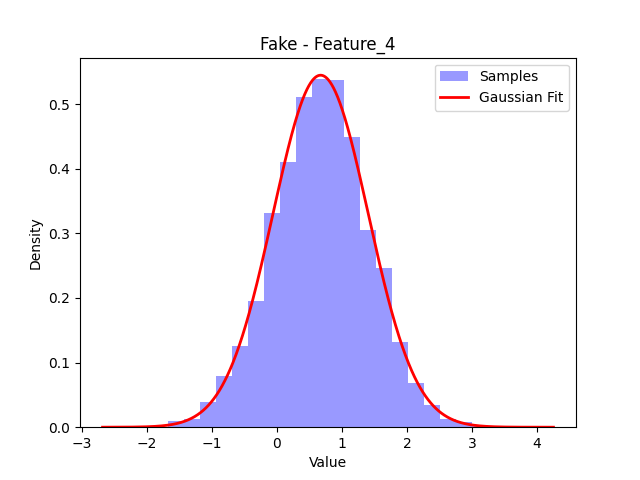
\includegraphics[width=0.48\linewidth]{fake_feature_4.png}
    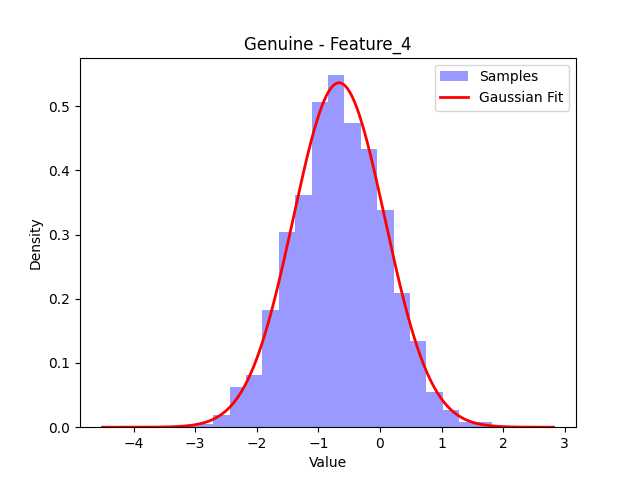
\includegraphics[width=0.48\linewidth]{genuine_feature_4.png}
    
    \caption{Examples of excellent Gaussian fits for Features 1-4 for both Fake (left) and Genuine (right) classes.}
    \label{fig:good_gaussian_fits}
\end{figure}

\subsection*{Question: Are there features for which the Gaussian model seems significantly less accurate?}

\subsubsection*{Empirical Results}
Yes, the Gaussian model is significantly inaccurate for **Features 5 and 6**, particularly within the Genuine class.

\begin{itemize}
    \item \textbf{Fake Class:} While technically unimodal, Features 5 and 6 exhibit very heavy tails. The rigid shape of the Gaussian bell curve underestimates these tails, resulting in a slight mismatch at the base of the distributions.
    \item \textbf{Genuine Class:} Features 5 and 6 are strictly \textbf{bimodal}. The empirical data is split into two distinct peaks separated by an empty "valley."
\end{itemize}

\subsubsection*{Theoretical Analysis}
The Gaussian distribution is mathematically constrained to be unimodal and symmetric. Applying MLE to the bimodal Genuine features forces the model to compute a global mean. For Feature 5, the ML mean is $-0.0417$, and for Feature 6, it is $0.0239$. The model places the absolute highest probability peak of the bell curve directly at these coordinates—which is exactly inside the empty valley where almost zero empirical samples exist. 

\subsubsection*{Motivation and Future Insights}
This visual proof of bimodality is critical for the architectural design of our classification system in subsequent laboratories. 

If we deploy a generative classifier based on a single Multivariate Gaussian (like the Standard or Tied MVG), the model will assign high log-likelihoods to test samples falling in the empty center of Features 5 and 6, guaranteeing misclassification. This geometrically proves why our dataset mathematically necessitates the use of a Gaussian Mixture Model (GMM) with multiple components, or non-linear kernel projections (like the RBF SVM), capable of wrapping multiple localized clusters simultaneously.

\begin{figure}[H]
    \centering
    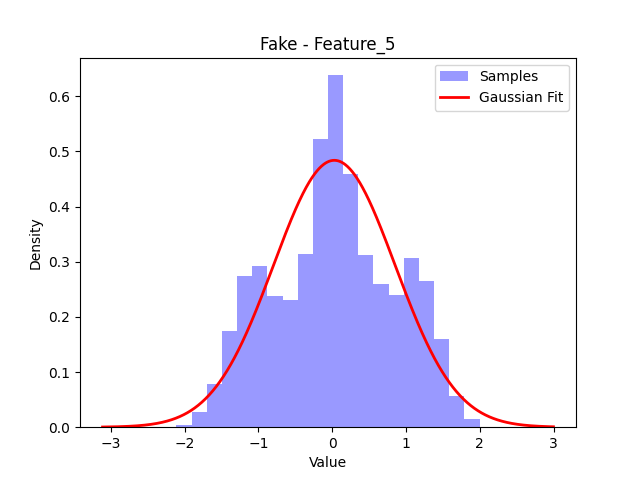
\includegraphics[width=0.48\linewidth]{fake_feature_5.png}
    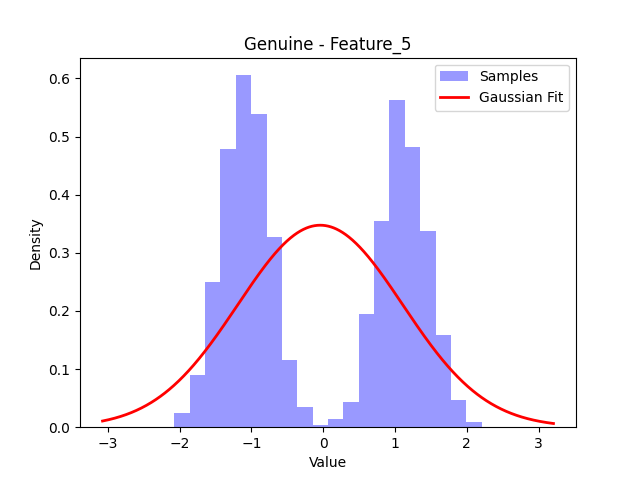
\includegraphics[width=0.48\linewidth]{genuine_feature_5.png}
    
    \vspace{0.3cm}
    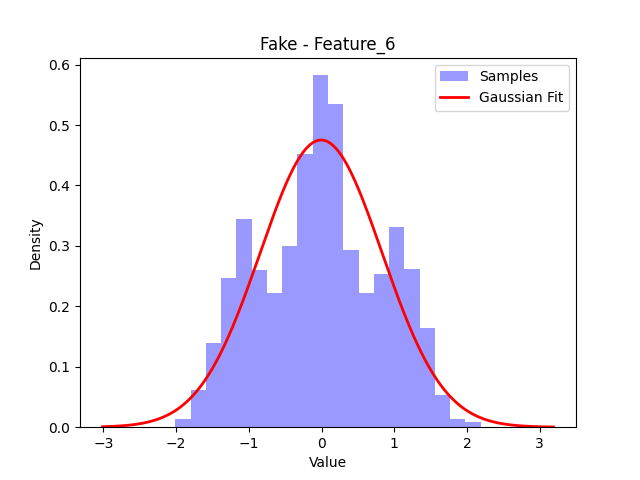
\includegraphics[width=0.48\linewidth]{fake_feature_6.png}
    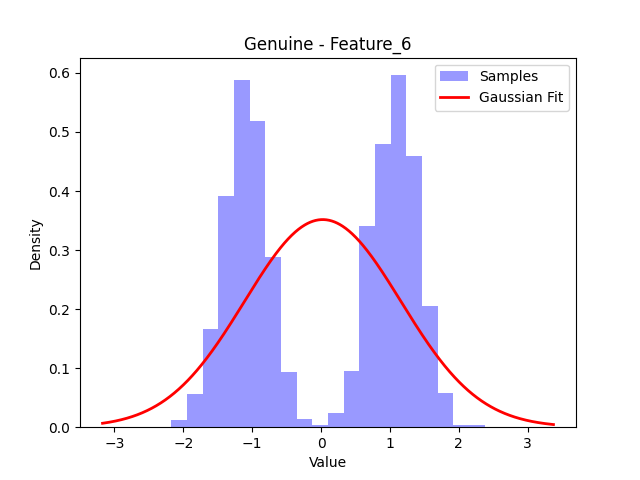
\includegraphics[width=0.48\linewidth]{genuine_feature_6.png}
    \caption{Examples of inaccurate Gaussian fits: Features 5 and 6. Note the catastrophic failure on the bimodal Genuine class (right).}
    \label{fig:bad_gaussian_fits}
\end{figure}

\end{document}